\documentclass{article}
\usepackage[margin=0.68in]{geometry}
\usepackage{minted}
\usepackage{xcolor}
\usepackage{fancyhdr}
\usepackage{graphicx}


\usemintedstyle{colorful}
\pagestyle{fancy}
\fancyhf{}
\rhead{adimail.github.io}
\lhead{Aditya Godse}

\definecolor{backcolour}{rgb}{0.95,0.95,0.92}

\begin{document}

% Program content begins
\section*{FizzBuzz - Javascript}
\begin{minted}[bgcolor=backcolour,linenos,frame=none]{js}
    const readline = require('readline');

    const rl = readline.createInterface({
      input: process.stdin,
      output: process.stdout
    });
    
    function what(num) {
      let result = num;
    
      if (num % 3 === 0) {
        result = "Fizz";
        if (num % 5 === 0) {
          result += " Buzz";
          return result;
        }
      }
    
      if (num % 5 === 0) {
        return "Buzz";
      }
    
      return result;
    }
    
    rl.question("Enter a number for n: ", (answer) => {
      const n = parseInt(answer);
    
      for (let i = 0; i <= n; i++) {
        console.log(what(i));
      }
    
      rl.close();
    });
    

\end{minted}
% Program content ends

% Capturing and including the program output as an image
\newpage

\section*{Program Output}
\begin{figure}[h]
    \centering
    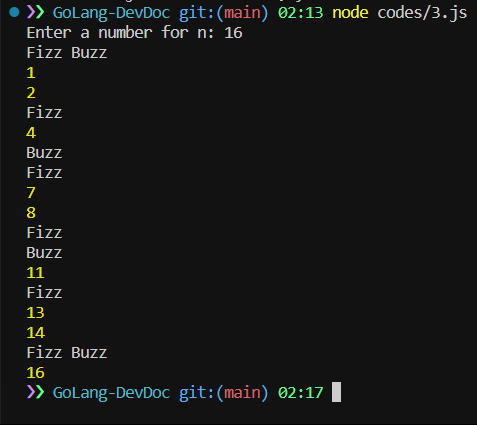
\includegraphics[width=1\textwidth]{./assets/fb.png}
    \caption{Program Output}
\end{figure}

\end{document}
